% Created 2020-10-25 So 23:03
% Intended LaTeX compiler: pdflatex
\documentclass[11pt]{scrartcl}
\usepackage[ngerman]{babel}
\usepackage{caption}
\usepackage[utf8]{inputenc}
\usepackage[T1]{fontenc}
\usepackage{graphicx}
\usepackage{grffile}
\usepackage{longtable}
\usepackage{wrapfig}
\usepackage{rotating}
\usepackage[normalem]{ulem}
\usepackage{amsmath}
\usepackage{textcomp}
\usepackage{amssymb}
\usepackage{capt-of}
\usepackage{MnSymbol}
\usepackage{mathtools}
\usepackage{setspace}
\usepackage{nicematrix}
\usepackage{listings}
\usepackage{pdfpages}
\usepackage[straightvoltages, european resistors, american inductors]{circuitikz}
\usetikzlibrary{arrows.meta}
\tikzset{FARROW/.style={arrows={-Triangle[angle=45:2.0mm]}}}


\renewcaptionname{ngerman}{\figurename}{Abb.}
\renewcaptionname{ngerman}{\tablename}{Tab.}



\author{David Keller, Moritz Woltron, Matthias Fottner}
\date{}
\title{Protokoll Übung 2}




\definecolor{darkspringgreen}{rgb}{0.09, 0.45, 0.27}    % Farbe für die Kommentare bei Listings
\lstset{
  language= Matlab,                     % Setzt die Sprache
  basicstyle=\scriptsize\ttfamily,     % Setzt den Standardstil
  % keywordstyle=\color{red}\bfseries,    % Setzt den Stil für Schlüsselwörter
  identifierstyle=\color{blue},        % Identifier bekommen keine gesonderte formatierung
  commentstyle=\color{darkspringgreen},        % Stil für Kommentare
  stringstyle=\ttfamily,             % Stil für Strings (gekennzeichnet mit "String")
  breaklines=true,             % Zeilen werden umgebrochen
  numbers=left,                 % Zeilennummern links
  numberstyle=\tiny,             % Stil für die Seitennummern
  frame=single,                 % Rahmen
  % backgroundcolor=\color{myGrey},     % Hintergrundfarbe
  % caption={Java-Code},             % Caption
  tabsize=2                % Größe der Tabulatoren
}




\begin{document}

\maketitle
\newcommand{\unit}[1]{\,\text{#1}}

\tableofcontents
\newpage
\section{Schaltplan mit allen Strömen, Spannungen und Knoten}

\begin{figure}[!htb]
  \centering
\hspace*{-40pt}
\begin{circuitikz}[scale=0.85]
  \clip (-4.5,-2.5) rectangle (16.5, 11);
  % create all nodes
  \draw node[label=left:$n_1$](n1) at (0,4)
        node[label=south east:$n_2$](n2) at (4,4)
        node[label=south east:$n_3$](n3) at (8,4)
        node[label=north:$n_4$](n4) at (4,8)
        node[label=left:$n_5$](n5) at (0,8)
        node[label=north:$a$](a) at (10,8)
        node[label=south:$b$](b) at (10,4);

  % draw all resistors
  \draw (n5) to[R=$R_1$, v={\color{blue}{$U_{R1}$}}, i={\color{red}{$I_{R1}$}}, o-o] (n1)
        (n1) to[short] ++ (0.4, 0) to[R=$R_2$, v={\color{blue}{$U_{R2}$}}, i={\color{red}{$I_{R2}$}}] ++ (2.7, 0 ) to[short] (n2)
        (n2) to[R=$R_3$, v={\color{blue}{$U_{R3}$}}, i={\color{red}{$I_{R3}$}}, o-o] (n4)
        (n2) to[short] ++ (0,-1) to[R=$R_4$, v={\color{blue}{$U_{R4}$}}, i={\color{red}{$I_{R4}$}}] ++ (0,-2.5) to[short] (4,0)
        (8,8) to[R=$R_5$, v={\color{blue}{$U_{R5}$}}, i={\color{red}{$I_{R5}$}}, o-o] (n3)
        (4,0) to[R=$R_6$, v={\color{blue}{$U_{R6}$}}, i={\color{red}{$I_{R6}$}}, o-] (8,0)
        (12,8) to[R=$R_7$, v={\color{blue}{$U_{R7}$}}, i={\color{red}{$I_{R7}$}}, o-o] (12,4);

  % draw sources
  \draw (0,0) to[cvsource={\color{blue}{$U_{S1}$}}, i>={\color{red}{$I_{S1}^?$}}] (n1)
        (n4) to[vsource, v_={\color{blue}{$U_{S2}$}}, i>_={\color{red}{$I_{S2}^?$}}] (n5)
        (n2) to[short, o-] ++ (0.5,0) to[isource, v>={\color{blue}{$U_{S3}^?$}}, i>={\color{red}{$I_{S3}$}}] ++ (3,0) to[short, -o] (n3)
        (15,4) to[isource, v>={\color{blue}{$U_{S4}^?$}}, i={\color{red}{$I_{S4}$}}] (15,8);

  % fill in wires
  \draw (0,0) to[short] (4,0);
  \draw (8,0) to[short] (8,4);
  \draw (n4) to[short] ++ (4,0);
  \draw (n3) to[short, -o] ++ (2,0) to[short] ++ (2,0) to[short] ++ (3,0);
  \draw (8,8) to[short, -o] ++ (2,0) to[short] ++ (2,0) to[short] ++ (3,0);

  % draw ground
  \draw (4,0) node[rground]{};

  % draw node currents
  \draw[european voltages, color=green!50!black] (n2) to[open, v=$U_{n2}$] (2.1,0)
                                                 (n1) to[open, v^=$U_{n1}$] (0.7,0)
                                                 (-1.5,8) to[open, v=$U_{n5}$] (-1.5,0);


  % \draw[FARROW, green!50!black] plot [smooth, tension=1] coordinates {(8.7,3.3) (9,-1) (4,-1)}
  \draw[FARROW, green!50!black] (8.6, 3.2) to[bend left=90, looseness=2] node[below right]{$U_{n3}$} (4.5,-1);
  \draw[FARROW, green!50!black] (3, 9) to[bend right=110, looseness=1.9] node[below left]{$U_{n4}$} (0,-0.5);

  % \draw [brown] (current bounding box.south west) rectangle (current bounding box.north east);
  % \draw[gray,step=0.25] (-6,-3) grid (16.5, 11);

\end{circuitikz}
\caption{Netzwerk mit allen eingezeichneten Strömen, (Knoten-)spannungen und Knoten}
\label{fig:net}
\end{figure}

\newpage

\section{Aufstellen des Gleichungssystems in Matrixform durch ``hinschauen''}
\subsection{Widerstände}
Zuerst wird die Admittanzmatrix durch hinschauen bestimmt.
Dazu werden auf der Hauptdiagonale alle den jeweiligen Knoten umgebenden Leitwerte addiert.
Auf der Nebendiagonale werden die Werte der zwischen den Knoten liegenden Widerstände als negativer Leitwert eingetragen.
Der Unbekanntenvektor besteht aus den Knotenspannungen, der Ergebnisvektor beträgt 0.

\NiceMatrixOptions{code-for-first-row = \color{orange},
  code-for-first-col = \color{orange}}
\begin{equation*}
 \text{Es gilt:} \quad G_n = \frac{1}{R_n}
\end{equation*}

\begin{align*}
  \renewcommand{\arraystretch}{1.5}
  \begin{bNiceArray}[first-row, first-col]{c:c:c:c:c}
          & n1 & n2 & n3 & n4 & n5 \\
          n1 & G_1+G_2 & -G_2 & 0 & 0 & -G_1 \\
          \hdottedline
          n2 & -G_2 & G_2 + G_3 + G_4 & 0 & -G_3 & 0 \\
          \hdottedline
          n3 & 0 & 0 & G_5 + G_6 & -G_5 & 0 \\
          \hdottedline
          n4 & 0 & -G_3 & -G_5 & G_3+G_5 & 0 \\
          \hdottedline
          n5 & -G_1 & 0 & 0 & 0 & G_1
        \end{bNiceArray}
   \begin{Bmatrix}
     U_{n1} \\
     U_{n2} \\
     U_{n3} \\
     U_{n4} \\
     U_{n5}
   \end{Bmatrix} =
  \begin{Bmatrix}
    0 \\
    0 \\
    0 \\
    0 \\
    0
  \end{Bmatrix}
\end{align*}
\subsection{Unabhängige Stromquelle $S3$}
Der bekannte Strom $I_{S3}$ der Stromquelle $S3$ fließt aus Knoten $n2$ (positiv) in den Knoten $n3$ (negativ)(vgl. Abb. \ref{fig:s3}).
Bringt man nun die Größe auf die andere Seite des Gleichungssystems,
so muss $I_{S3}$ im Lösungsvektor negativ bei $n2$ und positiv bei $n3$ sein.

\begin{figure}[!htb]
  \centering
\begin{circuitikz}
  \draw node[label=left:$n_2$](n2) at (0,0)
        node[label=right:$n_3$](n2) at (4,0);
  \draw (0,0) to[isource, v>={\color{blue}{$U_{S3}$}}, i={\color{red}{$I_{S3}$}}, o-o] (4,0);
\end{circuitikz}
\caption{freigestellte Stromquelle $S3$}
\label{fig:s3}
\end{figure}
Es ergibt sich folgende Änderung im Gleichungssystem:

\begin{align*}
  \renewcommand{\arraystretch}{1.5}
  \begin{bNiceArray}[first-row, first-col]{c:c:c:c:c}
    & n1 & n2 & n3 & n4 & n5 \\
    n1 & G_1+G_2 & -G_2 & 0 & 0 & -G_1 \\
    \hdottedline
    n2 & -G_2 & G_2 + G_3 + G_4 & 0 & -G_3 & 0 \\
    \hdottedline
    n3 & 0 & 0 & G_5 + G_6 & -G_5 & 0 \\
    \hdottedline
    n4 & 0 & -G_3 & -G_5 & G_3+G_5 & 0 \\
    \hdottedline
    n5 & -G_1 & 0 & 0 & 0 & G_1
  \end{bNiceArray}
                            \begin{Bmatrix}
                              U_{n1} \\
                              U_{n2} \\
                              U_{n3} \\
                              U_{n4} \\
                              U_{n5}
                            \end{Bmatrix} =
  \begin{Bmatrix}
    0 \\
    \color{red}{-I_{S3}} \\
    \color{red}{I_{S3}}\\
    0 \\
    0
  \end{Bmatrix}
\end{align*}

\subsection{Unabhängige Spannungsquelle $S2$ \color{green!50!black}{($\rightarrow +1$ Gleichung)}}
Bei der unabhängigen Spannungsquelle kommt mit dem Strom $I_{S2}^?$ eine unbekannte Größe hinzu.
Folglich muss auch eine weitere Gleichung im Gleichungssystem ergänzt werden.
Diese erhält man, indem die bekannte Quellspannung $U_{S2}$ mithilfe der Knotenspannungen ausgedrückt wird (vgl. Abb. \ref{fig:s2}):
\begin{equation*}
  {\color{blue}{U_{S2}}} = U_{n4} - U_{n5}
\end{equation*}
Beim Hinzufügen von $I_{S2}^?$ in den Unbekanntenvektor, muss auch die Strombilanz der Knoten $n4$ (positiv) und $n5$ (negativ) angepasst werden.

\begin{figure}[!htb]
  \centering
\begin{circuitikz}
  \draw node[label=left:$n_5$](n5) at (0,0)
        node[label=right:$n_4$](n4) at (4,0);
  \draw (4,0) to[vsource, v={\color{blue}{$U_{S2}$}}, i>={\color{red}{$I_{S2}^?$}}, o-o] (0,0);
\end{circuitikz}
\caption{freigestellte Spannungsquelle $S2$}
\label{fig:s2}
\end{figure}


\begin{align*}
  \renewcommand{\arraystretch}{1.5}
  \begin{bNiceArray}[first-row, first-col]{c:c:c:c:c:c}
    & n1 & n2 & n3 & n4 & n5 & \color{red}{I_{S2}^?}\\
    n1 & G_1+G_2 & -G_2 & 0 & 0 & -G_1 & 0\\
    \hdottedline
    n2 & -G_2 & G_2 + G_3 + G_4 & 0 & -G_3 & 0 & 0\\
    \hdottedline
    n3 & 0 & 0 & G_5 + G_6 & -G_5 & 0 & 0 \\
    \hdottedline
    n4 & 0 & -G_3 & -G_5 & G_3+G_5 & 0 & \color{red}{1} \\
    \hdottedline
    n5 & -G_1 & 0 & 0 & 0 & G_1 & \color{red}{-1} \\
    \hdottedline
    \color{red}{I_{S2}^?}   & 0 & 0 & 0 & \color{blue}{1} & \color{blue}{-1} & 0
  \end{bNiceArray}
                            \begin{Bmatrix}
                              U_{n1} \\
                              U_{n2} \\
                              U_{n3} \\
                              U_{n4} \\
                              U_{n5} \\
                              \color{red}{I_{S2}^?}
                            \end{Bmatrix} =
  \begin{Bmatrix}
    0 \\
    \color{red}{-I_{S3}} \\
    \color{red}{I_{S3}}\\
    0 \\
    0 \\
    \color{blue}{U_{S2}}
  \end{Bmatrix}
\end{align*}


\subsection{Stromgesteuerte Spannungsquelle $S1$ \color{green!50!black}{($\rightarrow +1$ Gleichung)}}\label{sec:completeMatrix}
Bei der stromgesteuerten Spannungsquelle $S1$ kommt die unbekannte Größe $I_{S1}^?$ hinzu.
Folglich muss auch hier das Gleichungssystem um eine Gleichung erweitert werden.
\begin{align*}
  U_{S1} &= \alpha \cdot I_{R3} \\
  I_{R3} &= G_3 (U_{n2} - U_{n4}) \\
  U_{S1} &= -U_{n1} \\
  \Longrightarrow -U_{n1} &= \alpha \cdot G_3 (U_{n2}- U_{n4}) \\
  0 &= \alpha \cdot G_3 (U_{n2} - U_{n4}) + U_{n1}
\end{align*}

\begin{figure}[!htb]
  \centering
  \begin{circuitikz}
    \draw node[label=left:$n_1$](n1) at (0,4)
          node[label=right:$n_2$](n2) at (6,0)
          node[label=right:$n_4$](n4) at (6,4);

          \draw (0,4) to[short, o-] ++ (2,0) to[cvsource, i={\color{red}{$I_{S1}^?$}}, v_<={\color{blue}{$U_{S1}$}}] (2,0) to[short, -o] (0,0)
          (2,0) node[rground]{}
          (6,0) to[short, o-] (4,0) to[R=$R_3$, i={\color{red}{$I_{R3}$}}] (4,4) to[short, -o] (6,4);
  \end{circuitikz}
  \caption{freigestellte stromgesteuerte Spannungsquelle $S1$ mit Steuerungsstrom $I_{R3}$}
  \label{fig:s1}
\end{figure}

\begin{align*}
  \renewcommand{\arraystretch}{1.5}
  \underbrace{\begin{bNiceArray}[first-row, first-col]{c:c:c:c:c:c:c}
    & n1 & n2 & n3 & n4 & n5 & \color{red}{I_{S2}^?} & \color{red}{I_{S1}^?}\\
    n1 & G_1+G_2 & -G_2 & 0 & 0 & -G_1 & 0 & -1\\
    \hdottedline
    n2 & -G_2 & G_2 + G_3 + G_4 & 0 & -G_3 & 0 & 0 & 0\\
    \hdottedline
    n3 & 0 & 0 & G_5 + G_6 & -G_5 & 0 & 0 & 0\\
    \hdottedline
    n4 & 0 & -G_3 & -G_5 & G_3+G_5 & 0 & \color{red}{1} & 0 \\
    \hdottedline
    n5 & -G_1 & 0 & 0 & 0 & G_1 & \color{red}{-1} & 0\\
    \hdottedline
    \color{red}{I_{S2}^?} & 0 & 0 & 0 & \color{blue}{1} & \color{blue}{-1} & 0 & 0 \\
    \hdottedline
    \color{red}{I_{S1}^?} & 1 & \alpha G_3 & 0 & -\alpha G_3 & 0 & 0 & 0
  \end{bNiceArray}}_{\text{A}}
                                                                               \underbrace{\begin{Bmatrix}
                                                                                 U_{n1} \\
                                                                                 U_{n2} \\
                                                                                 U_{n3} \\
                                                                                 U_{n4} \\
                                                                                 U_{n5} \\
                                                                                 \color{red}{I_{S2}^?} \\
                                                                                 \color{red}{I_{S1}^?}
                                                                               \end{Bmatrix}}_{\text{x}} =
  \underbrace{\begin{Bmatrix}
    0 \\
    \color{red}{-I_{S3}} \\
    \color{red}{I_{S3}}\\
    0 \\
    0 \\
    \color{blue}{U_{S2}} \\
    0
  \end{Bmatrix}}_{\text{b}}
\end{align*}

\subsection{Ausrechnen der Unbekanntenvektors $x$ } \label{sec:mat}
Indem man beide Seiten der Gleichung mit der Inversen $A^{-1}$ multipliziert, kann man nach $x$ auflösen.
\begin{equation*}
  x = A^{-1} b
\end{equation*}
Man erhält mithilfe von Matlab für $x$:
\begin{equation*}
  \renewcommand{\arraystretch}{1.5}
  x = \begin{Bmatrix}
    U_{n1} \\
    U_{n2} \\
    U_{n3} \\
    U_{n4} \\
    U_{n5} \\
    I_{S2}^? \\
    I_{S1}^? \\
  \end{Bmatrix} =
  \begin{Bmatrix}
    5,6140 \unit{V} \\
    -0,1754 \unit{V} \\
    23, 1579 \unit{V} \\
    20,8772 \unit{V} \\
    0,8772 \unit{V} \\
    -0,9474 \unit{A} \\
    1,5263 \unit{A}
  \end{Bmatrix}
\end{equation*}

\section{Thevenin-Quelle bezüglich der Klemmen $a$ und $b$}\label{sec:thev}
\subsection{$U_{Th}$}
Die Spannung $U_{Th}$ entspricht der Leerlaufspannung an den Klemmen $a$ und $b$ ($U_{ab,LL}$),
welche der Spannung $U_{R5}$ entspricht (vgl. Abb. \ref{fig:uth}).
Somit kann $U_{Th}$ mithilfe der gewonnenen Knotenspannungen aus Kapitel \ref{sec:mat} berechnet werden. Es gilt:
\begin{equation*}
  U_{Th} = U_{ab,LL} = U_{R5} = U_{n4} - U_{n3} = 20,8772 \unit{V} - 23,1579 \unit{V} = -2,2807 \unit{V}
\end{equation*}

\begin{figure}[!htb]
  \centering
\begin{circuitikz}
  \draw node[label=north:$n_4$](n4) at (0,4)
        node[label=north east:$n_3$](n3) at (0,0)
        node[label=north:$a$](a) at (2,4)
        node[label=south:$b$](b) at (2,0);

  \draw (-1,4) to[short, -o] (n4)
        (n4) to[R=$R_5$, v={\color{blue}{$U_{R5}$}}, o-o] (n3)
        (-1,0) to[short, -o] (n3)
        (n4) to[short, -o] (a)
        (n3) to[short, -o] (b)
        (n3) to[short] ++ (0,-0.5)
        (b) to[open, v<={\color{blue}{${U_{ab,LL} = U_{Th}}$}}] (a);
\end{circuitikz}
\caption{Spannungsbetrachtung an den Klemmen $a$ und $b$}
\label{fig:uth}
\end{figure}

\subsection{$I_{KS}$}
Bei $I_{KS}$ handelt es sich um eine weiter Unbekannte, deshalb muss das Gleichungssystem um eine weitere Gleichung
erweitert werden. Um den Kurzschluss zu simulieren, kann an den Klemmen $a$ und $b$ eine ideale Spannungsquelle mit
$0 \unit{V}$ Spannungsabfall angenommen werden (vgl. Abb. \ref{fig:iks}). Dieser Spannungsabfall entspricht $U_{R5}$,
und somit kann folgende Gleichung aufgestellt werden:

\begin{equation*}
  U_{R5} = U_{KS} = U_{n4} - U_{n3} = 0
\end{equation*}

\begin{figure}[!htb]
  \centering
  \begin{circuitikz}
    \draw node[label=north:$n_4$](n4) at (0,4)
          node[label=south east:$n_3$](n3) at (0,0)
          node[label=north:$a$](a) at (2,4)
          node[label=south:$b$](b) at (2,0);

    \draw (n4) to[R=$R_5$, v={\color{blue}{${U_{R5}=0 \unit{V}}$}}, o-o] (n3)
          (n4) to[short, -o] (a) to[short] ++ (2,0) to[vsource, v={\color{blue}{${U_{KS} = 0 \unit{V}}$}}, i>={\color{red}{$I_{KS}$}}] ++ (0,-4)
          (n3) to[short, -o] (b) to[short] ++ (2,0)
          (n3) to[short] ++ (0,-0.5)
          (n3) to[short] ++ (-1,0)
          (n4) to[short] ++ (-1,0);
  \end{circuitikz}
  \caption{Simulation des Kurzschlussstroms $I_{KS}$}
  \label{fig:iks}
\end{figure}

Der Kurzschlussstrom $I_{KS}$ muss als ausfließender Strom in Knoten $n_4$ und als zufließender Strom in Knoten $n_3$
ergänzt werden. Insgesamt ergibt sich folgendes Gleichungssystem:


\begin{align*}
  \renewcommand{\arraystretch}{1.5}
  \underbrace{\begin{bNiceArray}[first-row, first-col]{c:c:c:c:c:c:c:c}
      & n1 & n2 & n3 & n4 & n5 & \color{red}{I_{S2}^?} & \color{red}{I_{S1}^?} & \color{red}{I_{KS}}\\
      n1 & G_1+G_2 & -G_2 & 0 & 0 & -G_1 & 0 & -1 & 0\\
      \hdottedline
      n2 & -G_2 & G_2 + G_3 + G_4 & 0 & -G_3 & 0 & 0 & 0 & 0\\
      \hdottedline
      n3 & 0 & 0 & G_5 + G_6 & -G_5 & 0 & 0 & 0 & \color{red}{-1}\\
      \hdottedline
      n4 & 0 & -G_3 & -G_5 & G_3+G_5 & 0 & \color{red}{1} & 0 & \color{red}{1}\\
      \hdottedline
      n5 & -G_1 & 0 & 0 & 0 & G_1 & \color{red}{-1} & 0 & 0 \\
      \hdottedline
      \color{red}{I_{S2}^?} & 0 & 0 & 0 & \color{blue}{1} & \color{blue}{-1} & 0 & 0 & 0\\
      \hdottedline
      \color{red}{I_{S1}^?} & 1 & \alpha G_3 & 0 & -\alpha G_3 & 0 & 0 & 0 & 0 \\
      \hdottedline
      \color{red}{I_{KS}} & 0 & 0 & -1 & 1 & 0 & 0 & 0 & 0
    \end{bNiceArray}}_{\text{A}}
                                                                         \underbrace{\begin{Bmatrix}
                                                                             U_{n1} \\
                                                                             U_{n2} \\
                                                                             U_{n3} \\
                                                                             U_{n4} \\
                                                                             U_{n5} \\
                                                                             \color{red}{I_{S2}^?} \\
                                                                             \color{red}{I_{S1}^?} \\
                                                                             \color{red}{I_{KS}}
                                                                           \end{Bmatrix}}_{\text{x}} =
  \underbrace{\begin{Bmatrix}
      0 \\
      \color{red}{-I_{S3}} \\
      \color{red}{I_{S3}}\\
      0 \\
      0 \\
      \color{blue}{U_{S2}} \\
      0 \\
      0
    \end{Bmatrix}}_{\text{b}}
\end{align*}

Bei erneutem Auflösen nach $x$ und Ausrechnen der Gleichung mit Matlab erhält man für $x$:

\begin{equation*}
  x = \begin{Bmatrix}
    U_{n1} \\
    U_{n2} \\
    U_{n3} \\
    U_{n4} \\
    U_{n5} \\
    I_{S2}^? \\
    I_{S1}^? \\
    I_{KS} \\
  \end{Bmatrix} =
  \begin{Bmatrix}
    5,7143 \unit{V} \\
    1,7764 \cdot 10^{-15} \unit{V} \\
    21,4286 \unit{V} \\
    21,4286 \unit{V} \\
    1,4286 \unit{V} \\
    -0,8571 \unit{A} \\
    1,4286 \unit{A} \\
    -0,5714 \unit{A}
    \end{Bmatrix}
\end{equation*}
Der Kurzschlussstrom $I_{KS}$ entspricht somit $571,4 \unit{mA}$.

\subsection{$R_{Th}$ mithilfe von $U_{Th}$ und $I_{KS}$}\label{sec:var1}
Der Innenwiderstand $R_{Th}$ der Thevenin-Quelle entspricht dank der Quellenäquivalenz von Norton- und Thevenin-Quelle
dem Quotienten aus $U_{Th}$ und $I_{KS}$.
Somit ergibt sich:

\begin{equation*}
  R_{Th} = R_N = \frac{U_{Th}}{I_{KS}} = \frac{-2,2807 \unit{V}}{-0,5714 \unit{A}} = 3,9912 \unit{$\Omega$}
\end{equation*}

\subsection{$R_{Th}$ mithilfe von Testspannung $U_T$}

Um den Innenwiderstand der Thevenin-Quelle zu erhalten, werden zuerst alle unabhängigen Quellen im Netzwerk durch
deren idealen Innenwiderstand ersetzt. Zusätzlich wird an den Klemmen $a$ und $b$
eine frei wählbare Testspannung $U_T$ angelegt (vgl. Abb. \ref{fig:idealRq}).
Daraus ergibt sich ein unbekannter Teststrom $I_T^?$, der vom Knoten $n_4$ in den Knoten $n_3$ fließt.
Das Gleichungssystem aus Kapitel \ref{sec:completeMatrix} muss somit um eine weitere Gleichung ergänzt werden

\begin{equation*}
  U_T = U_{R5} = U_{n4} - U_{n3}
\end{equation*}

und man erhält folgende Matrixgleichung:

\begin{align*}
  \renewcommand{\arraystretch}{1.5}
  \underbrace{\begin{bNiceArray}[first-row, first-col]{c:c:c:c:c:c:c:c}
      & n1 & n2 & n3 & n4 & n5 & \color{red}{I_{S2}^?} & \color{red}{I_{S1}^?} & \color{red}{I_T^?}\\
      n1 & G_1+G_2 & -G_2 & 0 & 0 & -G_1 & 0 & -1 & 0 \\
      \hdottedline
      n2 & -G_2 & G_2 + G_3 + G_4 & 0 & -G_3 & 0 & 0 & 0 & 0\\
      \hdottedline
      n3 & 0 & 0 & G_5 + G_6 & -G_5 & 0 & 0 & 0 & \color{red}{-1} \\
      \hdottedline
      n4 & 0 & -G_3 & -G_5 & G_3+G_5 & 0 & \color{red}{1} & 0 & \color{red}{1} \\
      \hdottedline
      n5 & -G_1 & 0 & 0 & 0 & G_1 & \color{red}{-1} & 0 & 0 \\
      \hdottedline
      \color{red}{I_{S2}^?} & 0 & 0 & 0 & \color{blue}{1} & \color{blue}{-1} & 0 & 0 & 0 \\
      \hdottedline
      \color{red}{I_{S1}^?} & 1 & \alpha G_3 & 0 & -\alpha G_3 & 0 & 0 & 0 & 0 \\
      \hdottedline
      \color{red}{I_T^?} & 0 & 0 & -1 & 1 & 0 & 0 & 0 & 0
    \end{bNiceArray}}_{\text{A}}
                                                                         \underbrace{\begin{Bmatrix}
                                                                             U_{n1} \\
                                                                             U_{n2} \\
                                                                             U_{n3} \\
                                                                             U_{n4} \\
                                                                             U_{n5} \\
                                                                             \color{red}{I_{S2}^?} \\
                                                                             \color{red}{I_{S1}^?} \\
                                                                             \color{red}{I_{T}^?}
                                                                           \end{Bmatrix}}_{\text{x}} =
  \underbrace{\begin{Bmatrix}
      0 \\
      \color{red}{-I_{S3}} = 0\\
      \color{red}{I_{S3}} = 0\\
      0 \\
      0 \\
      \color{blue}{U_{S2}} = 0 \\
      0 \\
      \color{blue}{U_T}
    \end{Bmatrix}}_{\text{b}}
\end{align*}

\begin{figure}[!htb]
  \centering
  \hspace*{-40pt}
  \begin{circuitikz}[scale=0.85]
    \clip (-4.5,-2.3) rectangle (13.5, 10);
    % create all nodes
    \draw node[label=left:$n_1$](n1) at (0,4)
    node[label=south east:$n_2$](n2) at (4,4)
    node[label=south east:$n_3$](n3) at (8,4)
    node[label=north:$n_4$](n4) at (4,8)
    node[label=left:$n_5$](n5) at (0,8)
    node[label=north:$a$](a) at (10,8)
    node[label=south:$b$](b) at (10,4);

    % draw all resistors
    \draw (n5) to[R=$R_1$, v={\color{blue}{$U_{R1}$}}, i={\color{red}{$I_{R1}$}}, o-o] (n1)
    (n1) to[short] ++ (0.4, 0) to[R=$R_2$, v={\color{blue}{$U_{R2}$}}, i={\color{red}{$I_{R2}$}}] ++ (2.7, 0 ) to[short] (n2)
    (n2) to[R=$R_3$, v={\color{blue}{$U_{R3}$}}, i={\color{red}{$I_{R3}$}}, o-o] (n4)
    (n2) to[short] ++ (0,-1) to[R=$R_4$, v={\color{blue}{$U_{R4}$}}, i={\color{red}{$I_{R4}$}}] ++ (0,-2.5) to[short] (4,0)
    (8,8) to[R=$R_5$, v={\color{blue}{$U_{R5}$}}, i={\color{red}{$I_{R5}$}}, o-o] (n3)
    (4,0) to[R=$R_6$, v={\color{blue}{$U_{R6}$}}, i={\color{red}{$I_{R6}$}}, o-] (8,0);

    % draw sources
    \draw (0,0) to[cvsource={\color{blue}{$U_{S1}$}}, i>={\color{red}{$I_{S1}^?$}}] (n1)
    (n4) to[short, o-o] ++ (-1,0) to[short, v_={\color{blue}{${U_{S2} = 0 \unit{V}}$}}, i>={\color{red}{$I_{S2}^?$}}] ++ (-2,0) to[short, o-o] (n5)
    (n2) to[short, o-o] ++ (1,0) to[open, v>={\color{blue}{$U_{S3}^?$}}] ++ (2,0) to[short, o-o] (n3)
    (12,8) to[vsource, v={\color{blue}{$U_T$}}, i>={\color{red}{$I_T^?$}}, o-o] (12,4);

    % fill in wires
    \draw (0,0) to[short] (4,0);
    \draw (8,0) to[short] (8,4);
    \draw (n4) to[short] ++ (4,0);
    \draw (n3) to[short, -o] ++ (2,0) to[short] ++ (2,0);
    \draw (8,8) to[short, -o] ++ (2,0) to[short] ++ (2,0);

    % draw ground
    \draw (4,0) node[rground]{};

    % draw node currents
    \draw[european voltages, color=green!50!black] (n2) to[open, v=$U_{n2}$] (2.1,0)
    (n1) to[open, v^=$U_{n1}$] (0.7,0)
    (-1.5,8) to[open, v=$U_{n5}$] (-1.5,0);


    % \draw[FARROW, green!50!black] plot [smooth, tension=1] coordinates {(8.7,3.3) (9,-1) (4,-1)}
    \draw[FARROW, green!50!black] (8.6, 3.2) to[bend left=90, looseness=2] node[below right]{$U_{n3}$} (4.5,-1);
    \draw[FARROW, green!50!black] (3, 9) to[bend right=110, looseness=1.9] node[below left]{$U_{n4}$} (0,-0.5);

    % \draw [brown] (current bounding box.south west) rectangle (current bounding box.north east);
    % \draw[gray,step=0.25] (-6,-3) grid (16.5, 11);

  \end{circuitikz}
  \caption{Netzwerk mit idealen Innenwiderständen der unabhängigen Quellen und der Testspannung $U_T$ }
  \label{fig:idealRq}
\end{figure}

Legt man nun die Testspannung $U_T$ willkürlich auf $1 \unit{V}$ fest, so kann man das Gleichungssystem nach dem
x-Vektor auflösen und erhält mithilfe Matlabs den Wert des Stromes $I_T^?$.

\begin{equation*}
  I_T^? = -0,2505 \unit{A}
\end{equation*}

Die Situation kann wie in Abbildung \ref{fig:rth} dargestellt werden:

\begin{figure}[!htb]
  \centering
\begin{circuitikz}
  \draw (0,0) to[short, -o] (4,0)
        (0,0) to[short] (0,4) to[R=$R_{Th}$, v={\color{blue}{$U_{RTh}$}}, i={\color{red}{$I_T^?$}}, -o] (4,4)
              to[short] ++ (2,0) to[vsource, v={\color{blue}{$U_T$}}, i>={\color{red}{$I_T^?$}}] ++ (0,-4) to[short] ++ (-2, 0)
              node[label=north:$a$](a) at (4,4)
              node[label=south:$b$](b) at (4,0);
\end{circuitikz}
\caption{Testspannung am Innenwiderstand der Thevenin-Quelle}
\label{fig:rth}
\end{figure}

Es lässt sich also folgende Maschengleichung bestimmen:
\begin{equation*}
  U_{RTh} = - U_{T} = -1 \unit{V}
\end{equation*}

und letztlich der Widerstand $R_{Th}$ mithilfe des ohm'schen Gesetzes:
\begin{equation*}
  R_{Th} = \frac{U_{RTh}}{I_T^?} = \frac{-1 \unit{V}}{-0,2505 \unit{A}} = 3,9912 \unit{$\Omega$}
\end{equation*}

Dieser Wert deckt sich mit dem ausgerechneten Wert für $R_{Th}$ aus Kapitel \ref{sec:var1}.

\newpage

\section{Simulation in PSpice}
\subsection{Originalschaltung}
\begin{center}
  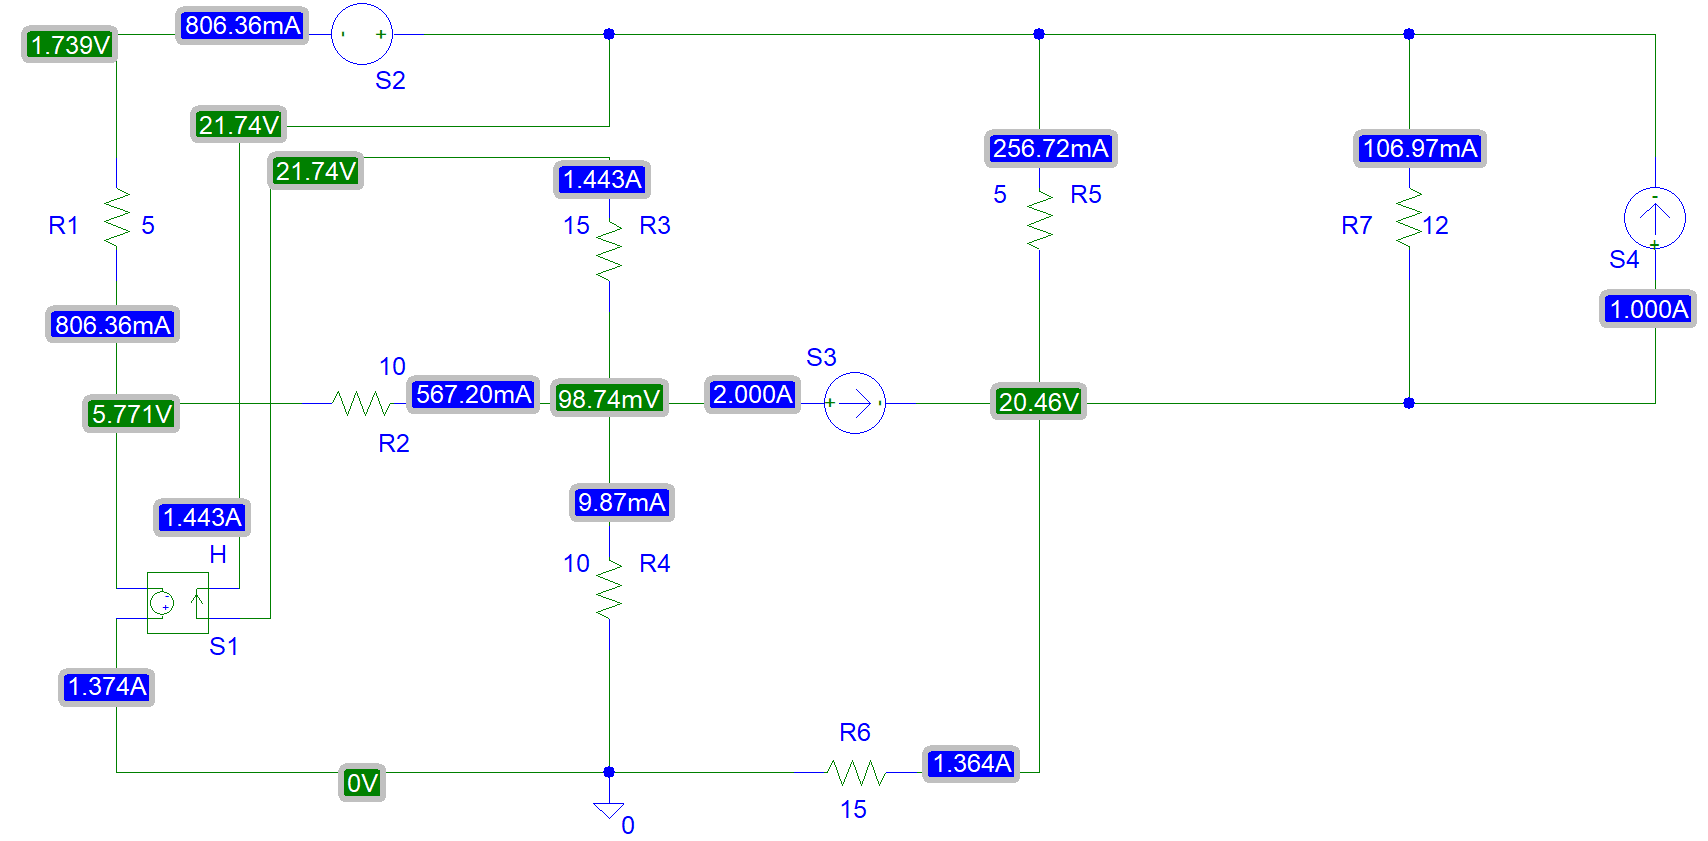
\includegraphics[width=1\linewidth]{./Assets/simulation_original}
  \captionof{figure}{PSpice-Simulation der Originalschaltung (vgl. Abb. \ref{fig:net})}
  \label{fig:sim_original}
\end{center}

\subsection{Thevenin-Quelle}
Bei der Simulation mit der Thevenin-Quelle wird das Netzwerk links von den Klemmen $a$ und $b$ durch eine
ideale Spannungsquelle mit der Spannung $U_{Th}$ und einem in Serie geschaltetem Innenwiderstand $R_{Th}$ ersetzt.
Die Werte hierfür wurden in Kapitel \ref{sec:thev} berechnet.
Der Schaltplan aus Abbildung \ref{fig:thev} liegt der Simulation zugrunde.

\begin{figure}[!htb]
\centering
  \begin{circuitikz}
    \draw (0,0) to[short, -o](4,0) to[short] ++ (6,0)
    to[isource, i={\color{red}{$I_{S4}$}}] ++ (0,4) to[short, -o] ++ (-6, 0) to[R=$R_{Th}$] (0,4)
    to[vsource, v={\color{blue}{$U_{Th}$}}] (0,0);
    \draw (6,4) to[R=$R_7$, v={\color{blue}{$U_{R7}$}}] (6,0);
    \draw node[label=north:$a$](a) at (4,4)
          node[label=south:$b$](b) at (4,0);
  \end{circuitikz}
  \caption{Ersatzschaltung mit Thevenin-Quelle}
  \label{fig:thev}
\end{figure}

\begin{center}
  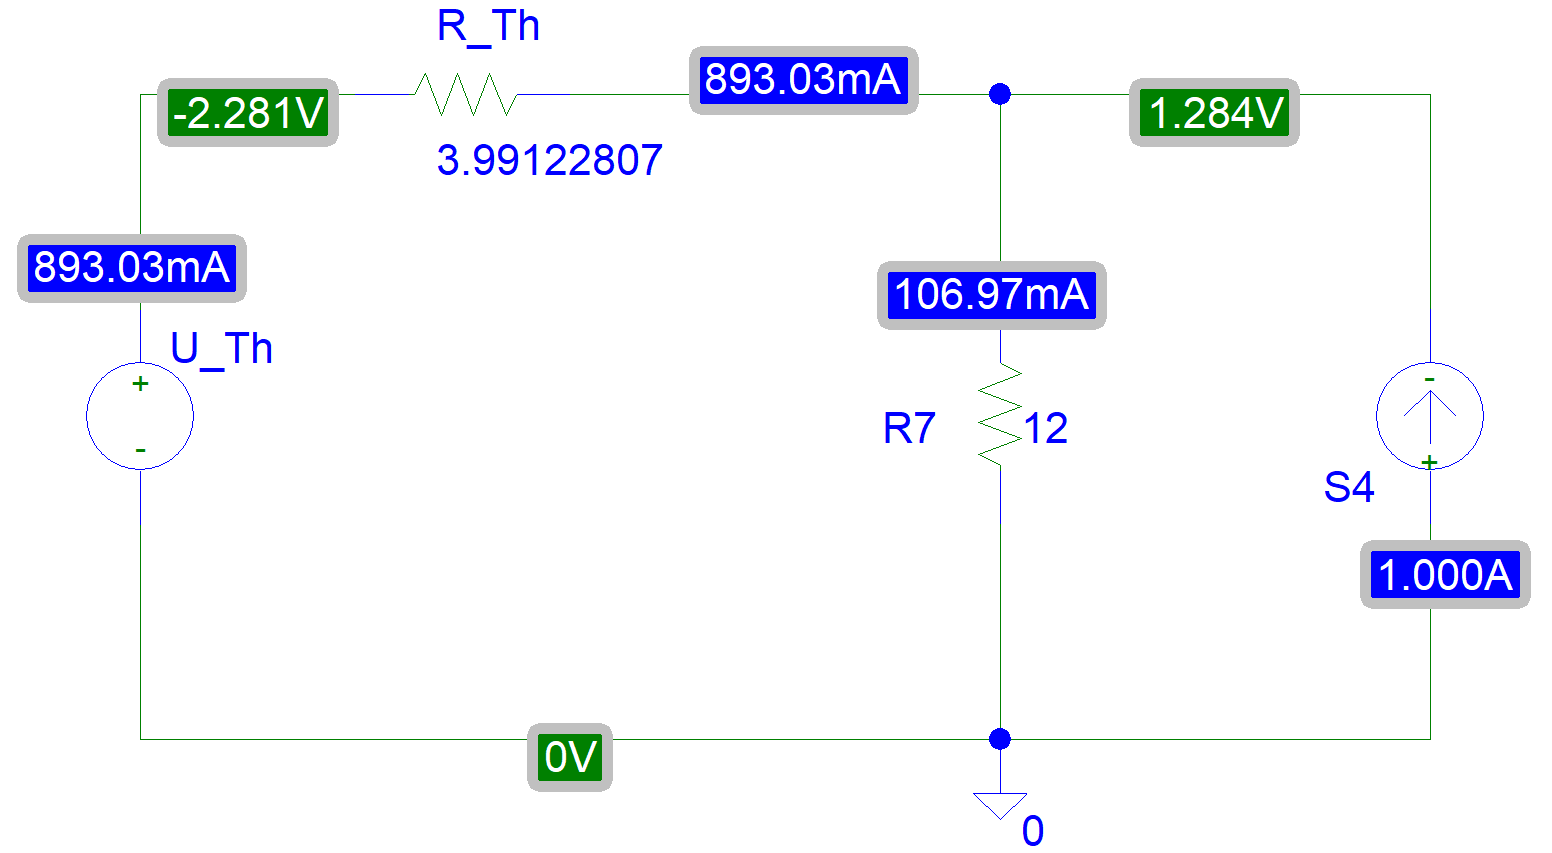
\includegraphics[width=1\linewidth]{./Assets/simulation_thevenin}
  \captionof{figure}{PSpice-Simulation der Thevenin-Ersatzschaltung (vgl. Abb. \ref{fig:net})}
  \label{fig:sim_thevenin}
\end{center}

\subsection{Vergleich der beiden Simulationen}

\end{document}